% Chapter 6
\section*{Preface}
In this chapter, performance of AIBs using various two-dimensional (2D) materials was explored. Nano structured molybdenum dichalcogenides (\ce{MoS2} and \ce{MoSe2}), graphitic carbon nitride (g-\ce{C3N4}), and electrospun tin oxide \ce{SnO2} fibers were tested as cathodes and their results have been reported. Prussian blue, which is a metal-organic framework (MOF), was also investigated as a cathode material. A comparison has been made between performance of bulk-\ce{MoSe2} and \ce{MoSe2} nanoflowers as cathodes in AIBs.7 
\pagebreak
\chapter{Aluminium batteries using various 2D materials as cathodes} 
\label{chap6} 
Recent development in teh field of two-dimensional (2D) materials has shown a lot of potential. Materials like graphene and its analogues, have remarkable electrochemical properties. These materials can be used in most of the energy storage devices such as batteries, supercapacitors, redox flow batteries, photovoltaics etc. In addition to their tunable chemical and physical properties, 2D materials possess different crystallographic structures and elemental compositions. For this reason, they find immense use as electrode materials in electrochemical energy storage devices\cite{wang_graphene_2009,bonaccorso_graphene_2015}. Furthermore, graphene and other 2D nanomaterials have a larger theoretical gravimetric capacity and also enable flexible and/or stretchable battery devices \cite{zhou_progress_2014}. 

\begin{figure}[h!]
  \centering
  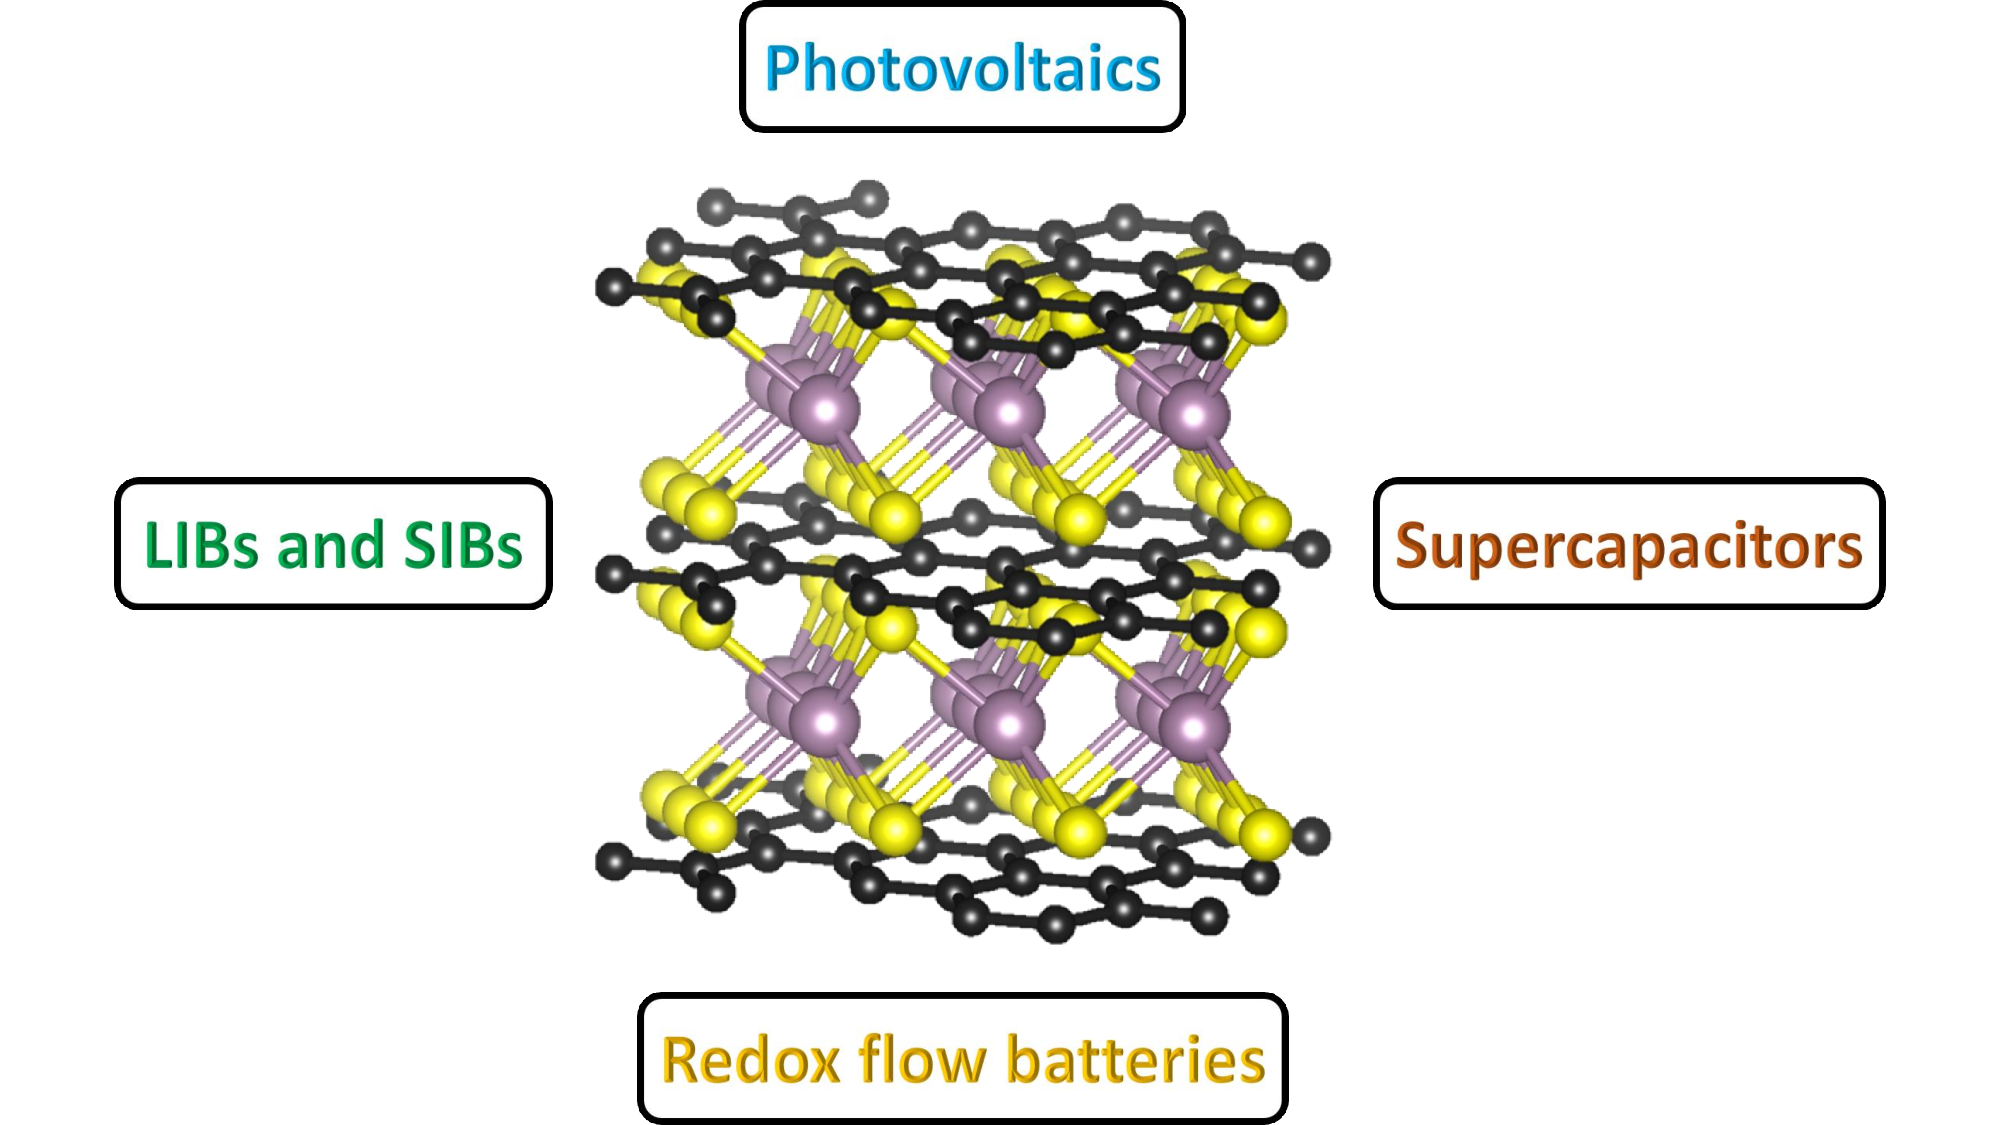
\includegraphics[width=\textwidth]{Figures/chap6fig/nanoTMDintro.pdf}
    \caption{.}
  \label{Figures/chap6fig:nanoTMDintro}
\end{figure}

\section{Nano-structured molybdenum sulfide and selenide}
Some TMDs such as \ce{TiS2} and exfoliated \ce{MoS2} flakes exhibit fast ionic conductivity as an electrochemically active material \cite{du_superior_2010,whittingham_electrical_1976}. A $\sim$750mAh g$^{-1}$ specific capacity was reported for restacked \ce{MoS2} single layers as a lithium-ion battery electrode. The restacking enlarged the c-axis parameter—the interlayer spacing, which increased the accessible surface area \cite{ammundsen_novel_2001}.
\subsection{Introduction}
Nano-sized materials increase the contact area between an electrode and electrolyte. The materials provide short path lengths for both ion diffusion and electron transport in comparison with bulk particles, which enhances the charge/ discharge rate. Since a shorter path length for electronic transport is created, materials having low electronic conductivity can also be utilised \cite{pitchai_nanostructured_2011}. The high surface area of nanomaterials allows large volume expansion/ contraction associated with ion transport and prevents cathode pulverisation, which leads to a longer cycle-life \cite{zhang_ultrathin_2015, cong_intrinsic_2015}. Transition metal dichalcogenides (TMDs) have a high surface area and potential to undergo redox reactions because they have multiple valencies. Nano TMDs have been widely explored as electrode materials since they have the potential to improve the electrochemical performance.  \\*
Nano TMDs have excellent electrochemical properties with a high surface-to-volume ratio. These materials have shown some remarkable performances in LIBs, sodium-ion batteries (SIBs), lithium-sulphur (Li-S) batteries, magnesium-ion batteries (MIBs), etc. In LIBs, graphene sheets and its analogues have shown a larger capacity over a graphite anode. The electrodes made of nanomaterials provide several advantages over bulk electrodes such as a high surface area, large void spaces and good electrical stability, which improves their lithium storage capability. Sheets of transition metal oxides also exhibit high specific capacity, and good stability. They are abundantly available, and are relatively easy to prepare. The storage of \ce{Li+} ions is based on a conversion reaction, where a reversible redox reaction takes place between lithium and transition metal cations \cite{reddy_metal_2013}. TMOs such as \ce{Fe2O3}, \ce{V2O5}, \ce{Nb2O5} and \ce{TiO2} have been used as anodes in LIBs. Fe2O3, for example has a very high theoretical specific capacity of 1006 mAh g$^{-1}$. This is why TMDs and TMOs have been considered as the next generation of electrode materials in batteries. With the rapid progress in research on 2D nanomaterials, large-scale preparation of nano-structured materials at a low cost can be expected for practical applications in the near future. \\*

\begin{sidewaystable}
\centering
\caption{Summary of performances of 2D materials in various energy storage devices.} \label{table1}
\begin{tabular}{ |p{1.5cm}|p{3.5cm}|p{4.5cm}|p{4.5cm}|p{4.5cm}|}
 \hline 
\textbf{Ref.} & \textbf{Electrode} & \textbf{Electrolyte} & \textbf{Storage capacity} & \textbf{Cycle performance} \\ 
\hline
\cite{acerce_metallic_2015-1} & {\center{Metallic 1T \ce{MoS2}}} & 0.5M \ce{H2SO4}, \ce{Li2SO4}, \ce{K2SO4} or KCl or EMIm \ce{BF4} & Volumetric capacitance: 400-700 F cm$^{-3}$ & >90\% retained after 5000 cycles\\
\cite{zhao_flexible_2015} & MXene/CNTs & 1M \ce{MgSO4} & Volumetric capacitance: 350F cm$^{-1}$ & No degradation after 10000 cycles at 10 A g$^{-1}$\\
\cite{hu_hierarchical_2015} & \ce{TiO2} & 1M \ce{LiPF6} in a 1: (v:v) mixture of ethylene carbonate and dimethyl carbonate & Specific capacity: 182 mAh g$^{-1}$ at 5C & 87.9\% retained after 400 cycles at 5C \\
\cite{cao_preparation_2013} & \ce{MoS2}/graphene & 1M \ce{LiPF6} in a 1:1 (V:v) mix of ethylene carbonate and dimethyl carbonate & Specific capacity: 466 mAh g$^{-1}$ at 4 A g$^{-1}$ & 566 mAh g$^{-1}$ retained after 50 cycles at 0.5 A g$^{-1}$ \\
\cite{ding_facile_2012} & \ce{TiO2}/CNT \ce{SnO2}/CNT & 1M \ce{LiPF6} in a 1:1 (w:w) mix of ethylene carbonate and dimethyl carbonate & Specific capacity: 320 mAh g$^{-1}$ for \ce{TiO2}, 580 mAh g$^{-1}$ for \ce{SnO2} at 0.4 A g$^{-1}$ & 93.8\% retained after 120 cycles for \ce{TiO2}, 72.4\% retained after 40 cycles at 0.4 A g$^{-1}$ for \ce{SnO2}\\
\cite{xie_mos2/graphene_2015} & \ce{MoS2}/rGO & 1M \ce{NaClO4} in a 1:1 (V:v) mix of ethylene carbonate and dimethyl carbonate & Specific capacity: 350 mAh g$^{-1}$ at 0.64 A g$^{-1}$ & 227 mAh g$^{-1}$ retained after 300 cycles at 0.32 A g$^{-1}$ \\
\hline
\end{tabular}
\end{sidewaystable}

\subsection{Experimental methods}
The materials were obtained from Tohoku university and used as received. 
%Before adding sulfur, pristine \ce{MoO3} (Wako chemicals) was ball-milled for 4 hours. 1 mmol of ascorbic acid (Wako chemicals) as a reducing agent was dissolved in 5 ml of water and the mixture was magnetically stirred for at least 20 minutes under air. Subsequently, 1 mmol of S powder (Sigma-Aldrich) and 0.3 mmol of ball-milled \ce{MoO3} were placed in the reactor. Lastly, 5 ml of ascorbic acid aqueous solution was injected into the reactor vessels containing the powder mixture. The sealed reactor was kept at 400$^{\circ}$C in a tube furnace for 30 minutes. After heating, the samples were collected in the same procedure as above.

\subsection{Results and discussion}
\ce{MoS2} and \ce{MoSe2} nanoflowers achieved a discharge capacity of 55 mAh g$^{-1}$ and 65 mAh g$^{-1}$ at a current rate of 50 mA g$^{-1}$ respectively. Figure \ref{Figures/chap6fig:MoX2YNCDCsCEs}a and b shows the charge and discharge curves at different current rates ranging from 50 to 1500 mA g$^{-1}$ with cutoff voltages at 0.2 and 2.35 V. Figure \ref{Figures/chap6fig:MoX2YNCDCsCEs}c and d displays the rate performance of both cells. It was observed that at higher current, the capacity of the cell decreased, while the coulombic efficiency increased. At 1500 mA g$^{-1}$, both Al/\ce{MoS2} and Al/\ce{MoSe2} displayed a capacity of $\sim$20 mAh g$^{-1}$ with 99.5\% coulombic efficiency. The discharge capacity increased to 50 mAh g$^{-1}$ after 120 cycles at a slower current rate of 50 mA g$^{-1}$. However, it was observed that the discharge curve for both nano-structured cathodes was a smooth line without any plateaus or bends. If we recall Chapter\ref{chap4} (Figure \ref{Figures/chap4fig:MoX2CDCCV}), bulk molybdenum dichalcogenides showed distinct voltage bends and plateaus. It seemed that the electron transfer process was a surface-based adsorption and not an intercalation process. Since both \ce{MoS2} and \ce{MoSe2} nanoflowers display similar specific capacities at similar current rates after 120 cycles, it can be assumed that the chloroaluminates were reversibly adsorbed on their surface. 

\begin{figure}[h!]
  \centering
  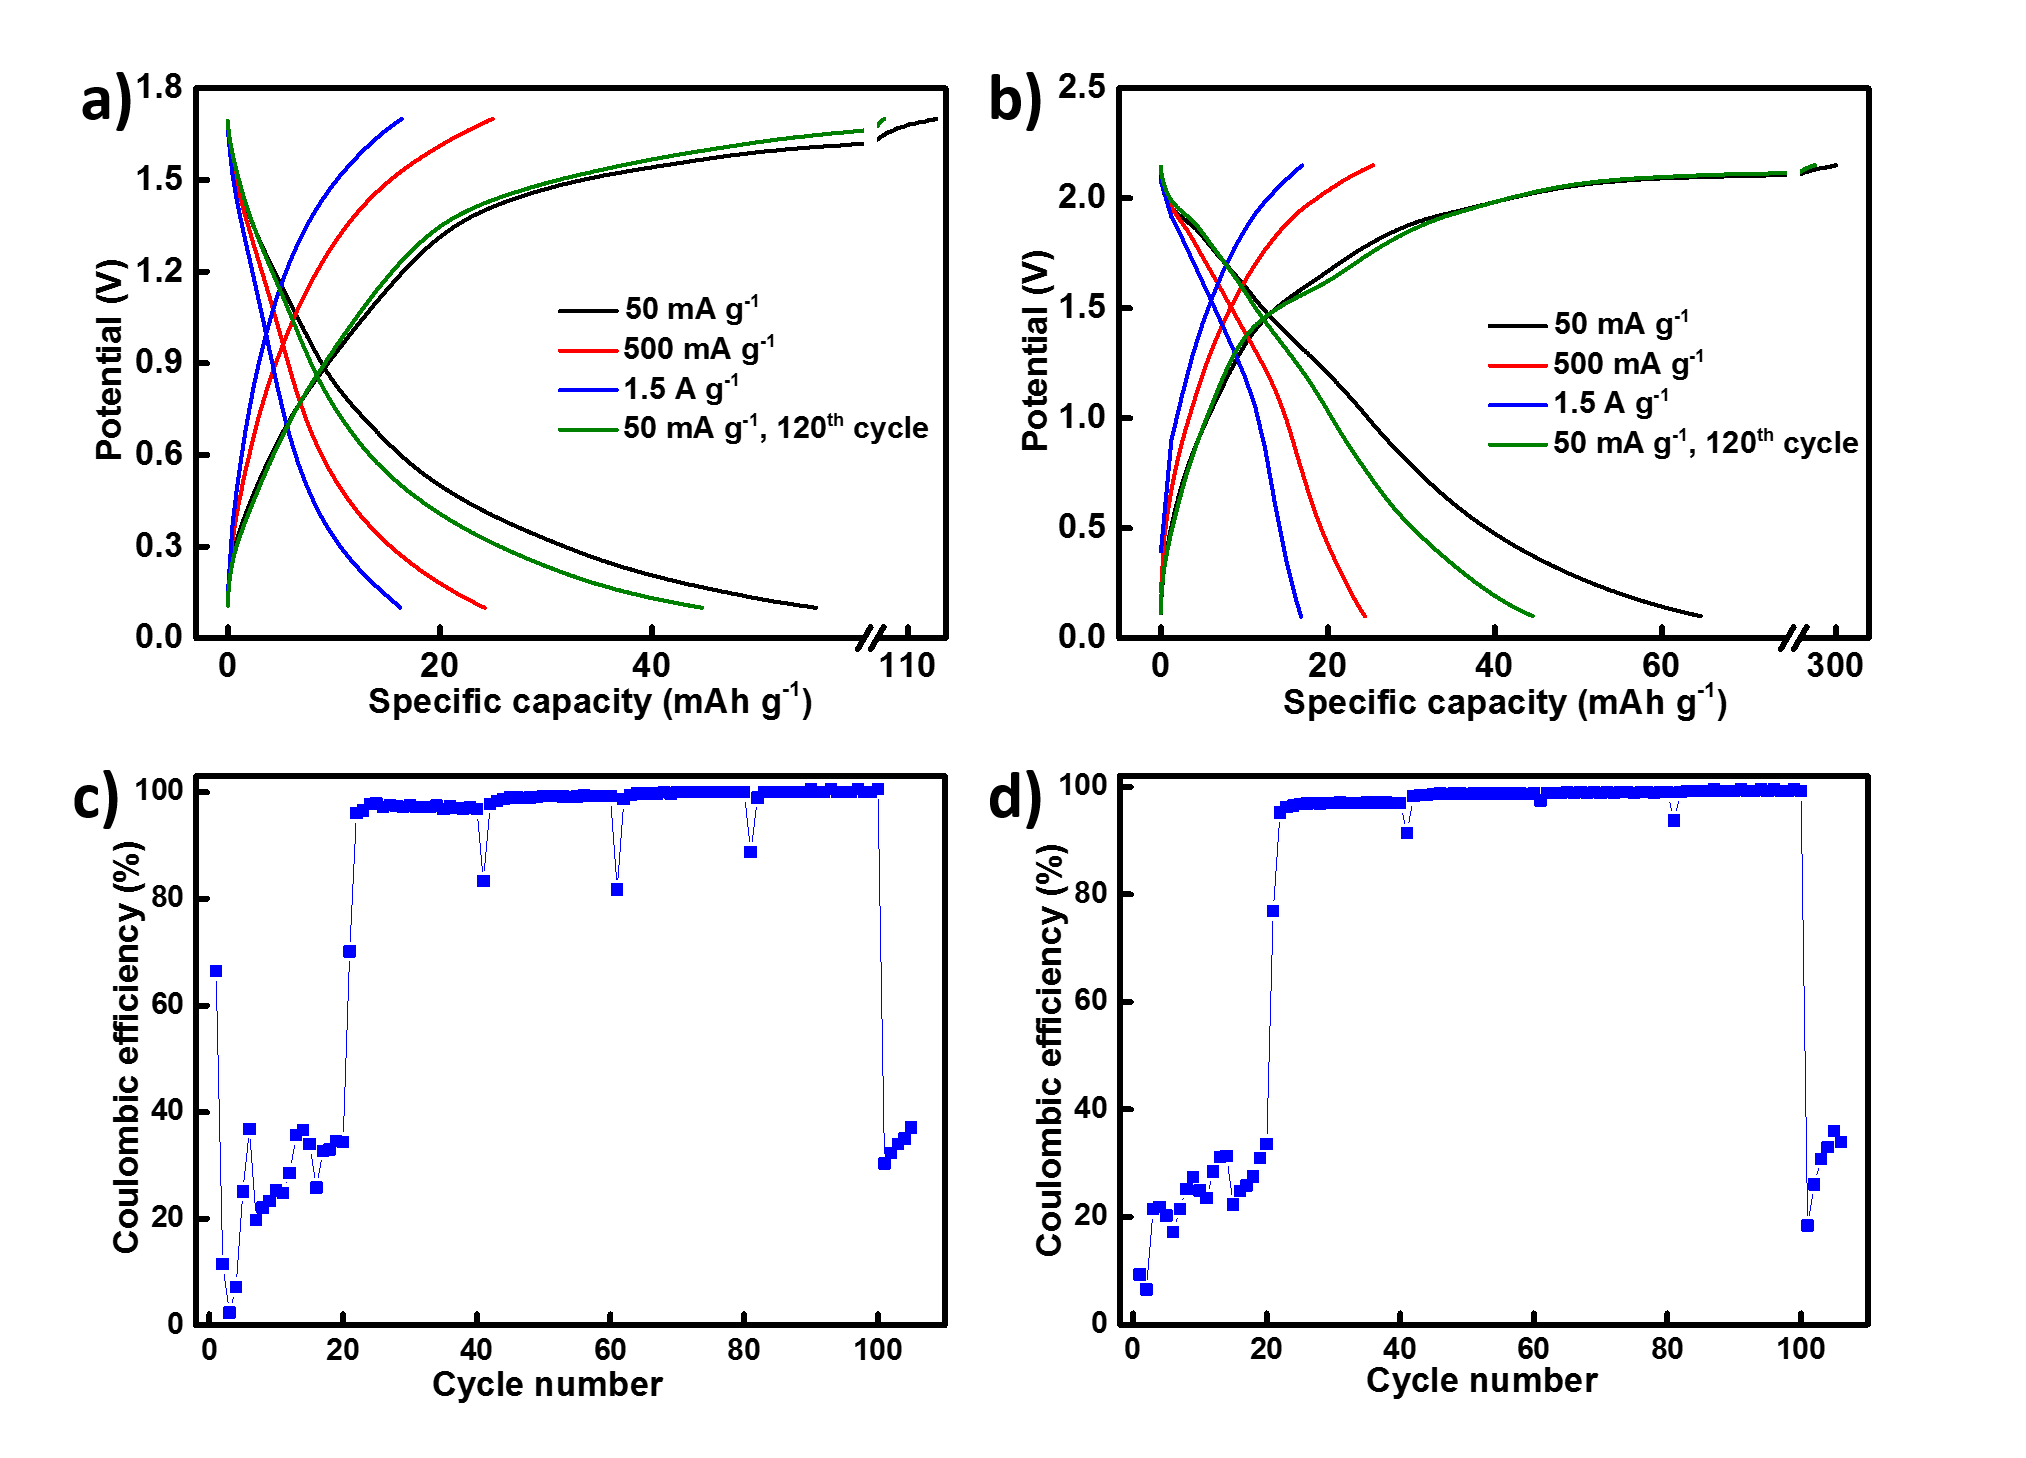
\includegraphics[width=\textwidth]{Figures/chap6fig/MoX2YNCDCsCEs}
    \caption{Galvanostatic charge and discharge curves of a) Al/\ce{MoS2} and b) \ce{MoSe2} cell at various current densities. Long-term stability test of c) Al/\ce{MoS2} and d) \ce{MoSe2} cells. All capacity was recorded between charging and discharging voltages of 0.2 and 2.35 V.}
  \label{Figures/chap6fig:MoX2YNCDCsCEs}
\end{figure}

\begin{figure}[th!]
\centering

\includegraphics[width=0.75\textwidth]{Figures/chap6fig/MoSe2YNCV}
\caption{\textit{Ex-situ} X-ray diffraction patterns of \ce{SnO2} cathode in a pristine (black), charged (green) and discharged (red) state.}
\label{Figures/chap6fig:MoSe2YNCV}
\end{figure}
Another interesting observation was the CV scan of nano-\ce{MoSe2}. The bulk and nano \ce{MoSe2} displayed their oxidation and reduction peaks at similar voltages. 

A schematic of the mechanism is displayed in Figure \ref{Figures/chap6fig:nanbulkmox2}.    

\begin{figure}[h!]
  \centering
  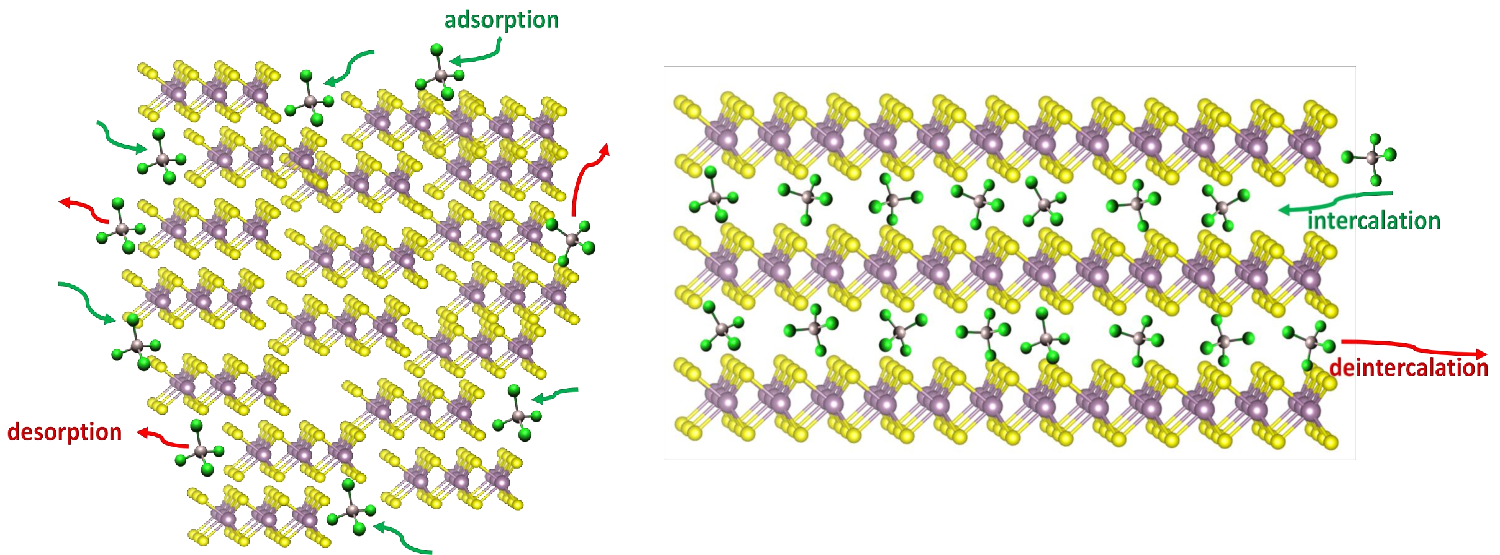
\includegraphics[width=\textwidth]{Figures/chap6fig/nanbulkmox2.pdf}
    \caption{Schematic illustration of the mechanisms followed by \ce{MoX2} nanoflowers (left) and bulk material (right).}
  \label{Figures/chap6fig:nanbulkmox2}
\end{figure}

While intercalation of chloroaluminates takes place in bulk \ce{MoX2}, the insertion of ions seems less probable on the nanoscale. Although the interlayer distance remains the same (6.5\AA) for both, the nano-sized structure obstructs a continuous intercalation process. Because of their high surface area, nanoflowers follow a capacitor-like charge storage, where the layers did not undergo any expansion and the specific capacities come from non-faradaic reactions where \ce{AlCl4-} anions electrostatically get absorbed and desorbed at their surfaces.

\section{Tin oxide}

\subsection{Introduction}

\begin{figure}[th!]
  \centering
  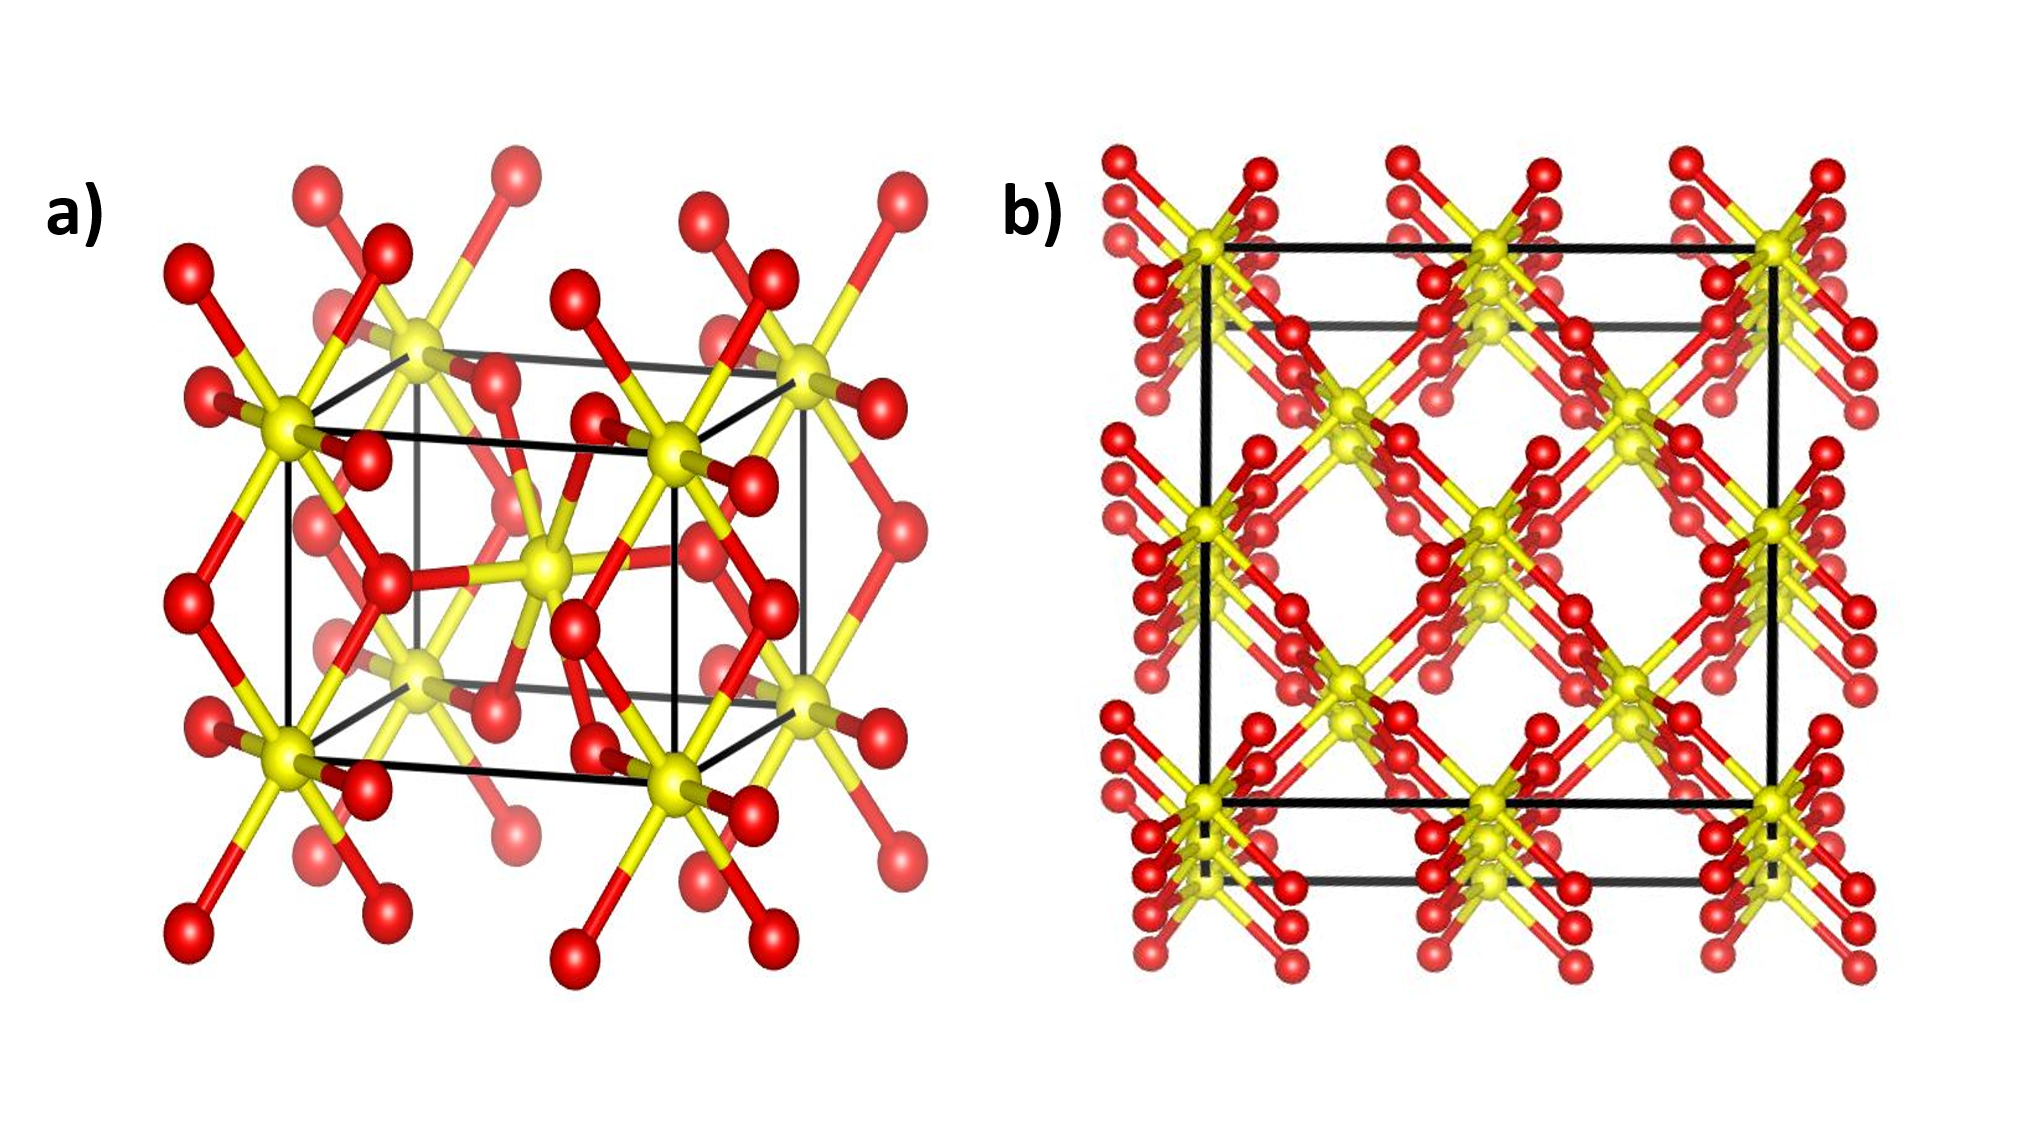
\includegraphics[width=\textwidth]{Figures/chap6fig/SnO2crys}
    \caption{Crystal structure of \ce{SnO2}. a) Tetragonal unit cell with space group P4/nmm and space group number 129. b) Top view of the crystal lattice.}
  \label{Figures/chap6fig:SnO2crys}
  \end{figure}
  
Due to its high theoretical capacity ($\approx$ 782mAh g$^{-1}$) and safe handling, \ce{SnO2} has been a popular choice in energy storage devices  \cite{idota_tin-based_1997}. They are a safer choice as compared to metallic lithium. Unfortunately, the major disadvantage of these materials is the large volume change during lithium insertion/extraction. A volume change of $\sim$360\% in pure tin metal causes an internal strain. Whittingham \textit{et al.} showed that pure tin foil (bulk) can be cycled as 600 mAh g$^{-1}$ for 10 to 15 cycles \cite{yang_anodes}. However, the expansion and contraction of the anode during cycles causes pulverisation and increases of the cell impedance. Consequently, due to the loss of electronic contact between active materials and the current collector, the capacity of the cells decreases after 15 cycles. Formation of \ce{Li2O} in addition to the volume expansion, further deteriorates the battery performance \cite{zhao_tin-based_2016}. Equation 1 describes \ce{Li2O} formation and Equation 2 describes the large volume variation \cite{park_effect_2008}.

\begin{center}
\ce{SnO2} + 4\ce{Li+} + 4\ce{e-} $\longrightarrow$ 2\ce{Li2O} + \ce{Sn} (1) 
\end{center}
\begin{center}
x\ce{Li} + x\ce{e-} + y\ce{Sn} $\longrightarrow$ \ce{Li_{x}Sn}  (2)
\end{center}

Since \ce{Li2O} is electrochemically inactive and non-conductive, it is also responsible for the large initial irreversible capacity. It has been reported that \ce{Li2O} can be decomposed via structural modifications of \ce{SnO2} on a nanoscale. Tin-based anodes have demonstrated improved electrochemical performance and cycle life and a controlled expansion process during lithiation.  

\begin{figure}[th!]
\centering
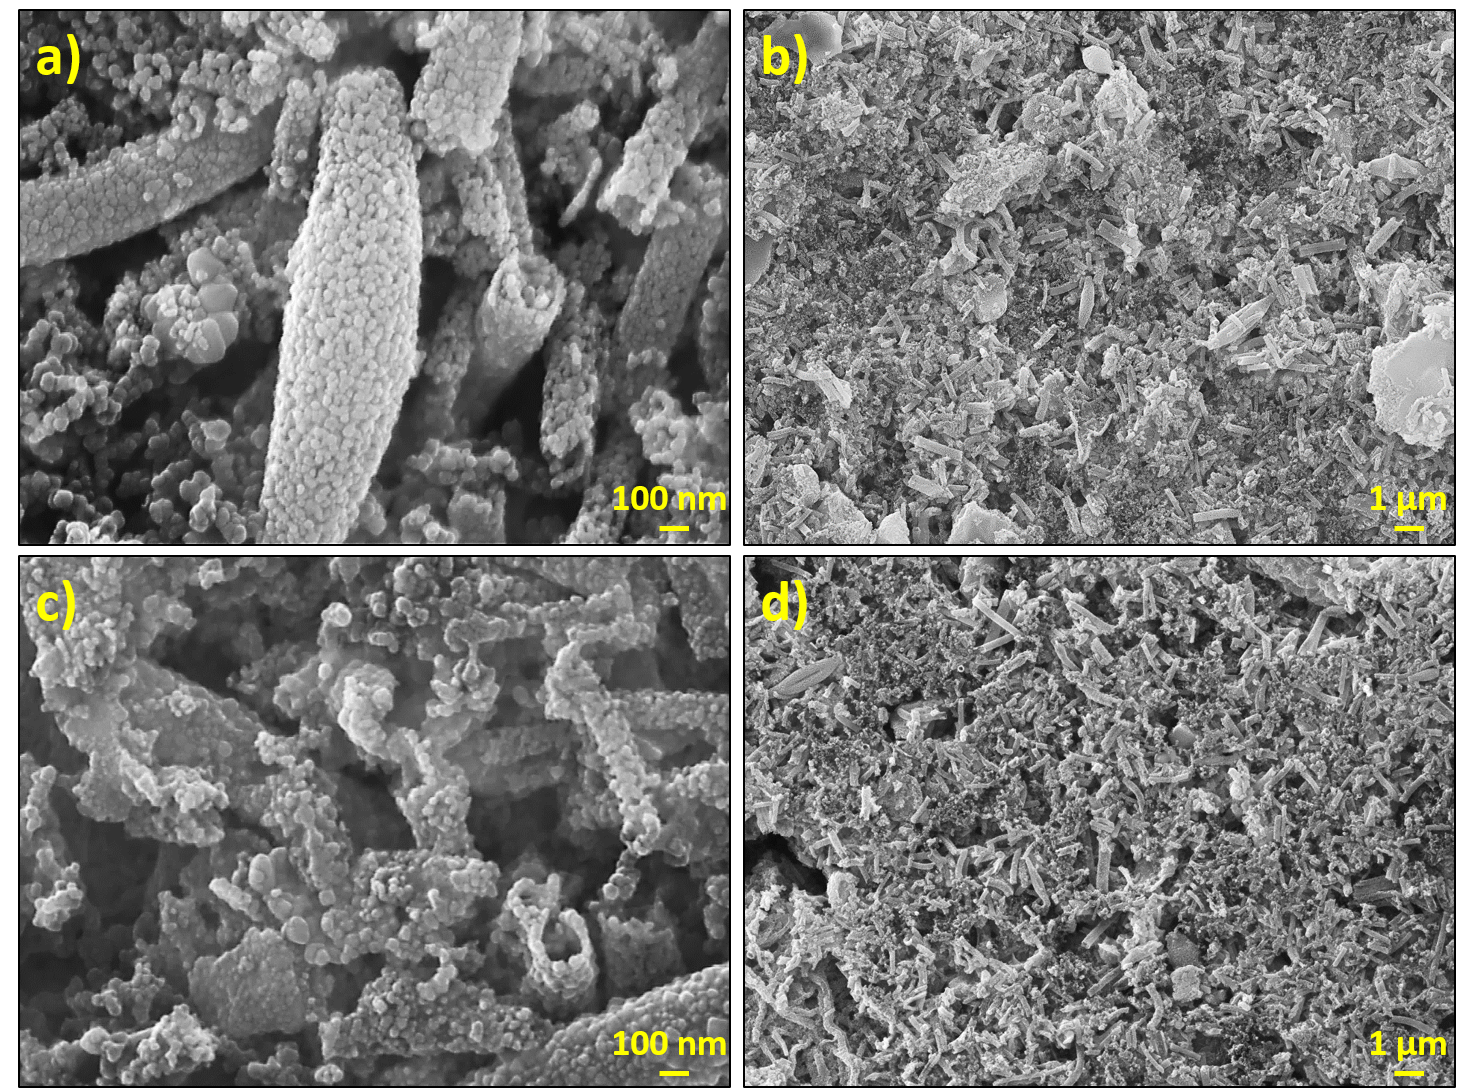
\includegraphics[width=\textwidth]{Figures/chap6fig/SnO2SEM}
\caption{SEM images of a,c)pristine and b,d) cycled \ce{SnO2} cathode.}
\label{Figures/chap6fig:SnO2SEM}
\end{figure}

It has been proposed that adding carbonaceous materials to \ce{SnO2} increases its surface area, which makes more active sites available for lithiation \cite{navarro-suarez_2d_nodate}. It also controls the volume expansion/shrinkage. Furthermore, it improves the conductivity of the material \cite{nowak_composites_2018}. Several nano-structured tin-based materials such as nano-rods \cite{liu_direct_2009}, nano-belts \cite{duan_single_2005}, nano-wires \cite{huang_situ_2010}, nano-tubes \cite{wang_large-scale_2011} have been synthesised and tested as electrodes. In this chapter, \ce{SnO2} fibers were obtained via  \enquote{electrospinning}. Electrospinning is a technique that uses electric force to draw charged threads of polymer solutions in the order of a few 100 nanometers. A schematic is illustrated in Figure \ref{Figures/chap6fig:electrospinning}. The topography and orientation of the fibers can be controlled by modifying a few parameters such as voltage, pump speed, nozzle thickness, etc. 

\begin{figure}[th!]
\centering
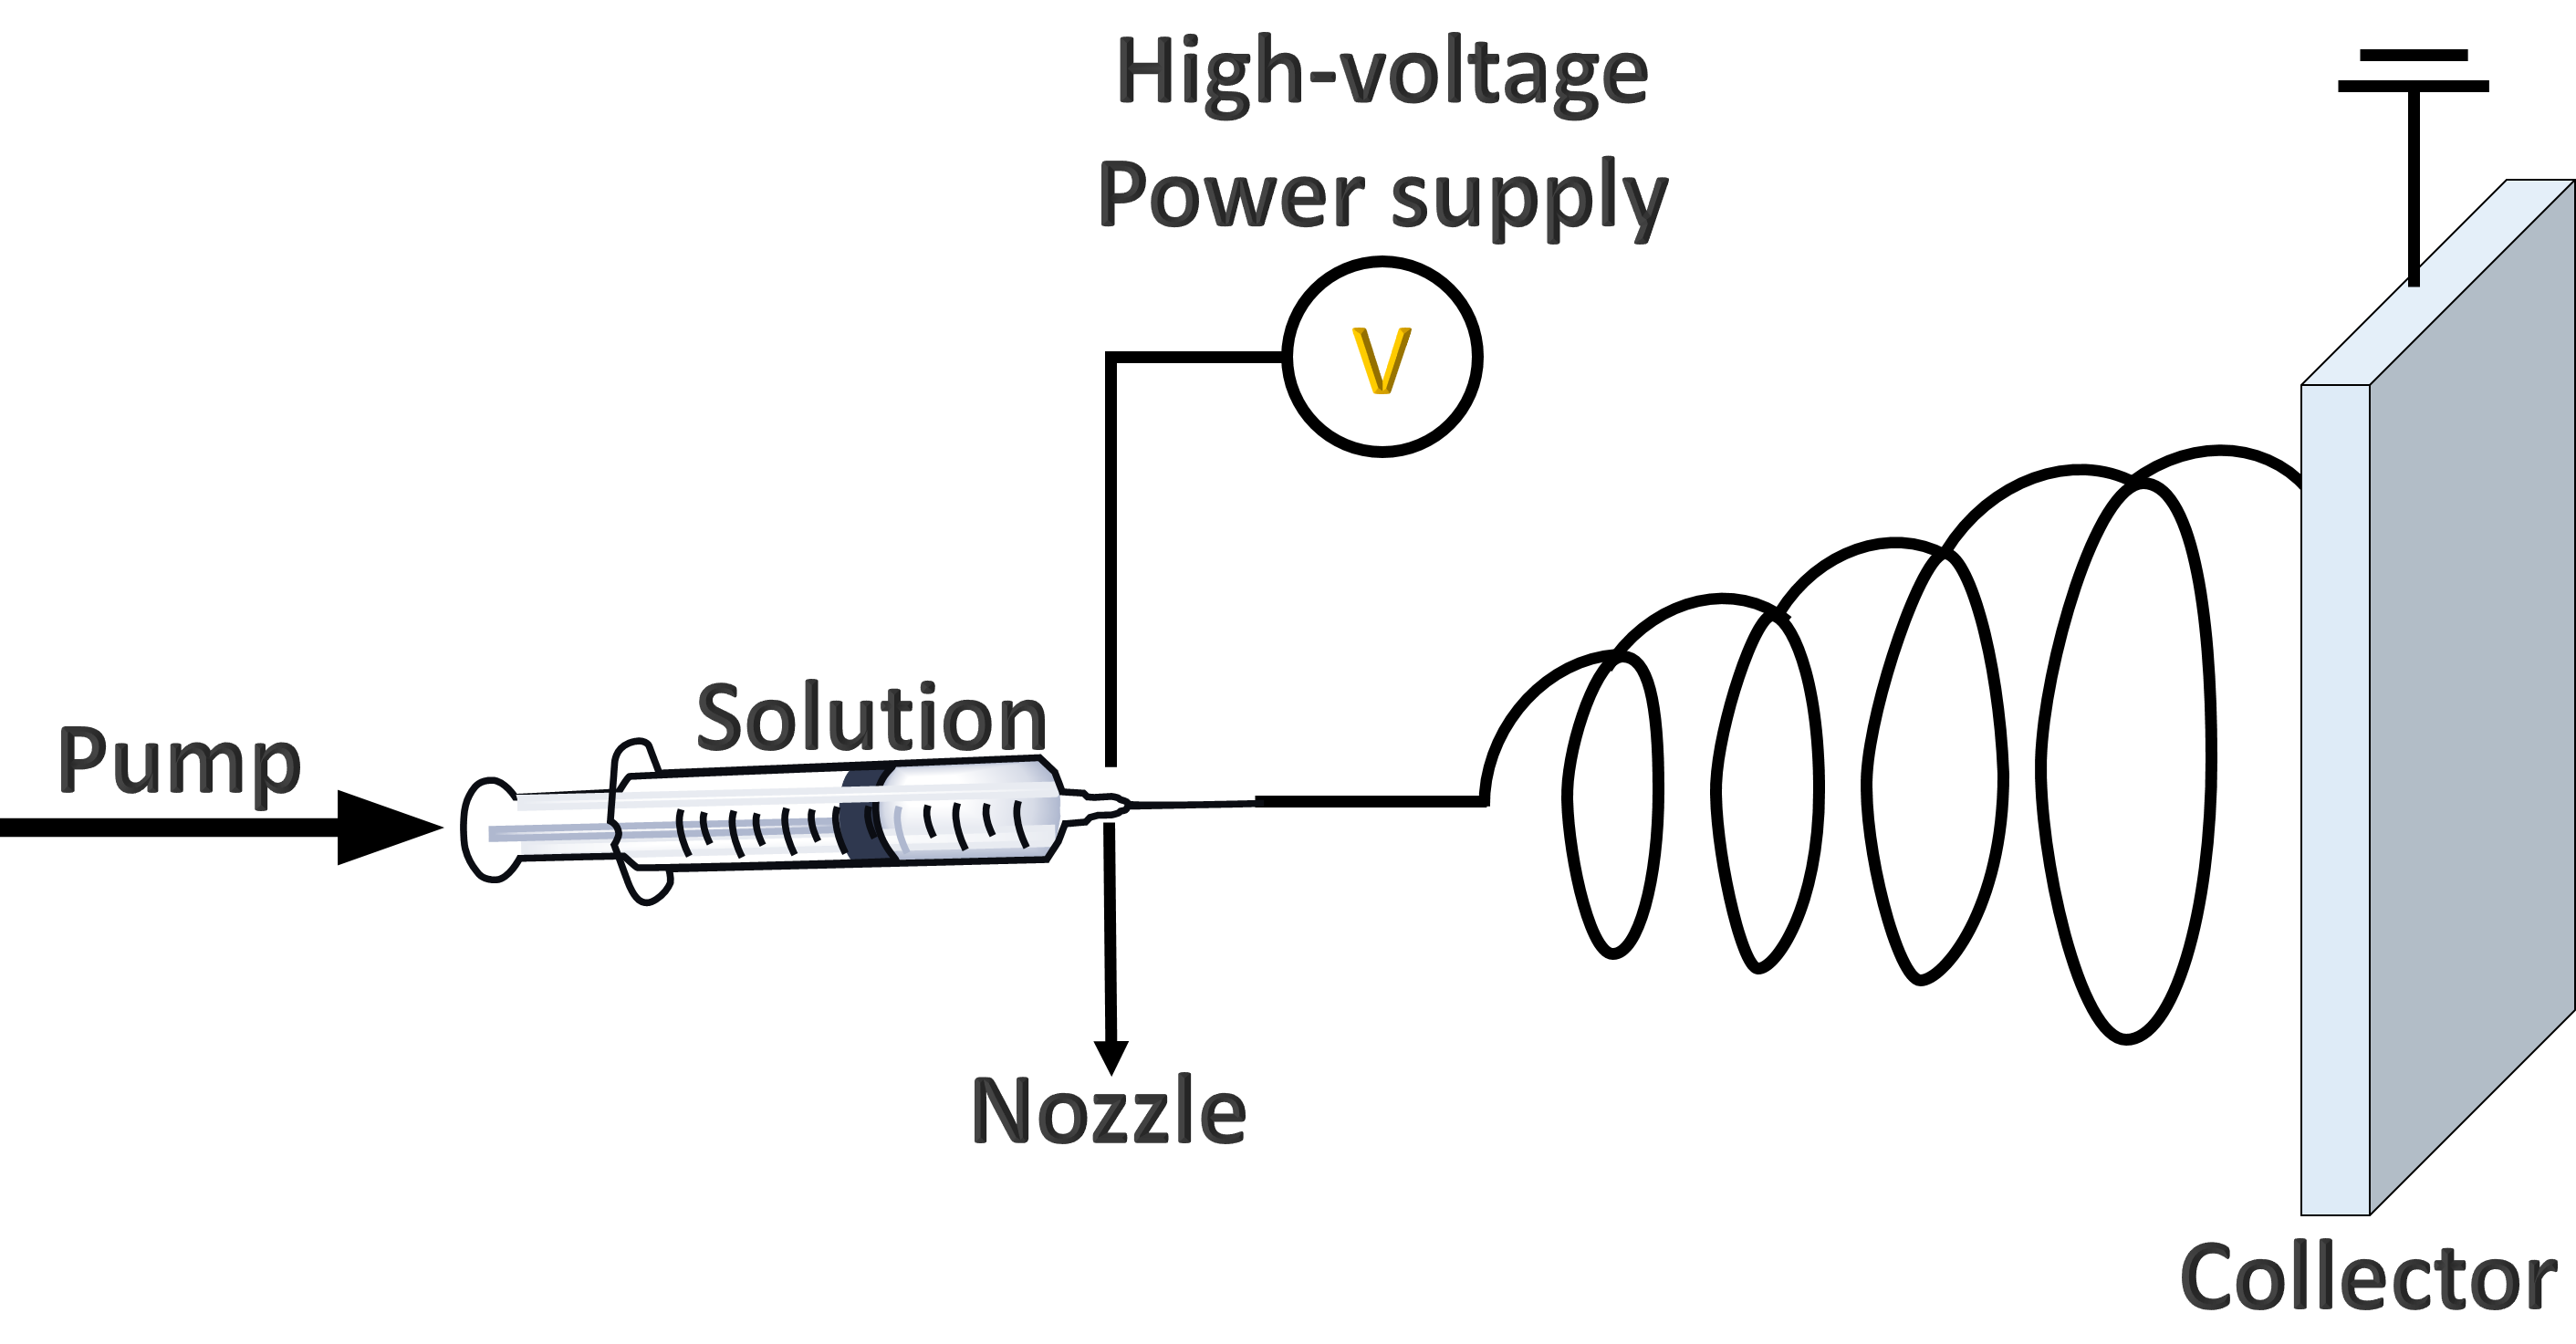
\includegraphics[width=\textwidth]{Figures/chap6fig/electrospinning}
\caption{SEM images of a,c)pristine and b,d) cycled \ce{SnO2} cathode.}
\label{Figures/chap6fig:electrospinning}
\end{figure}

\subsection{Experimental methods}
The material was obtained from University of Montpellier, France and was used as received. 

\subsection{Results and discussion}
To evaluate the electrochemical properties of the designed Al-ion cell, a galvanostatic discharge/charge reaction was performed at the cell voltage of 0.2-2.35 V at current densities ranging from 50-1500 mA g$^{-1}$. Figure \ref{Figures/chap6fig:SnO2perfCDC} displays the voltage vs. specific capacity plot of the AIB. The curves demonstrate a well defined discharge plateau at $\sim$ 0.55 V. In the first cycle, the battery achieved a capacity of 105 mAh g$^{-1}$, which decreased to 50 mAh g$^{-1}$ after 120 cycles. Coulombic efficiency of the cell decreased with every cycle. It stabilised at $\sim$60\%. Since the discharge capacity decreases after every cycle,\ce{SnO2} as a cathode material in an AIB probably undergoes similar volumetric changes like in LIBs.   

 \begin{figure}[th!]
  \centering
  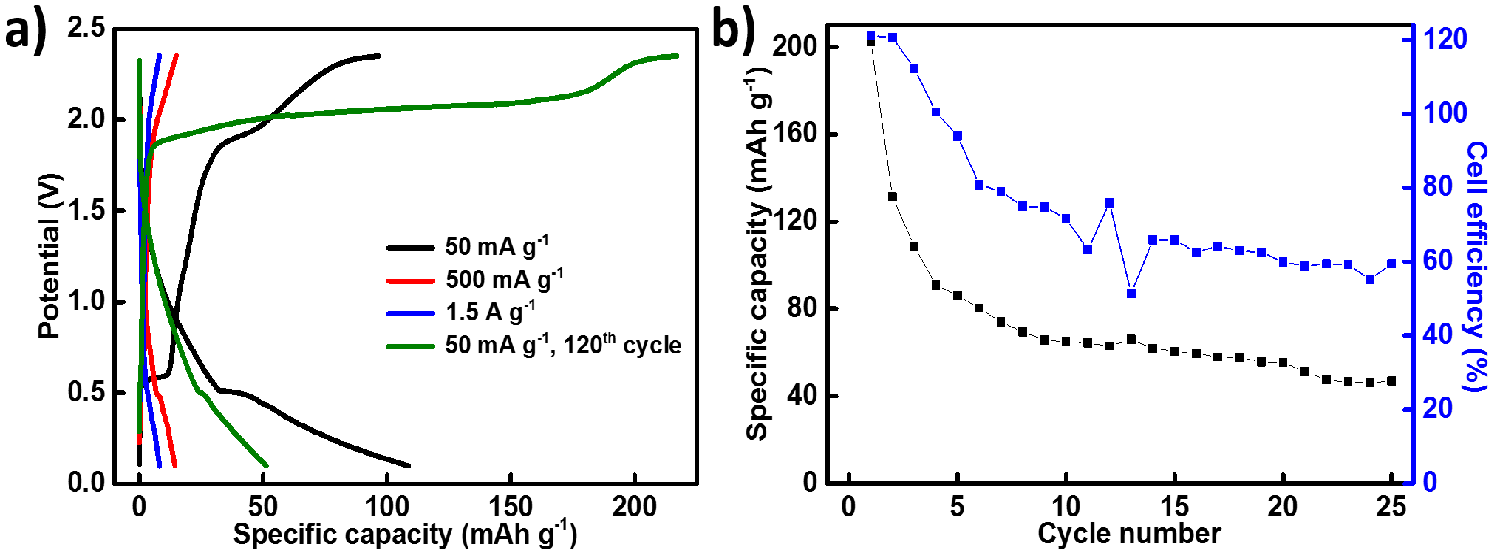
\includegraphics[width=\textwidth]{Figures/chap6fig/SnO2perfCDC.pdf}
    \caption{Galvanostatic charge and discharge curve of an Al/\ce{SnO2} cell at various current rates.}
  \label{Figures/chap6fig:SnO2perfCDC}
\end{figure}

\begin{figure}[th!]
\centering
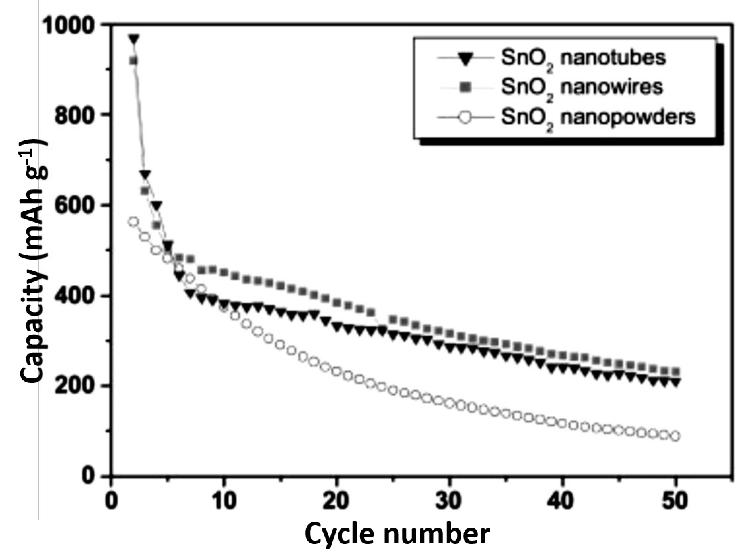
\includegraphics[width=0.75\textwidth]{Figures/chap6fig/sno2pap.pdf}
\caption{The cyclic performance of \ce{SnO2} nanomaterials in lithium-ion batteries up to the fiftieth cycle at a current density of 100 mA g$^{-1}$. Capacity of the materials decreases with every cycle due to expansion of \ce{SnO2}, which leads to cathode pulverisation and capacity fading.}
\label{Figures/chap6fig:sno2pap}
\end{figure}
However, the X-ray diffraction patterns in Figure \ref{Figures/chap6fig:SnO2XRD} look alike after charge and discharge except a shoulder that develops in the charged and discharged cathodes at 2$\thets$ value of 22$^{\circ}$. The fibers maintain their long-range order even after cycles. SEM images in Figure \ref{Figures/chap6fig:SnO2SEM} display the cathode morphology before and after cycles. The fibers seem to retain their tubular structure after charge/discharge, although a few fibres show signs of damage in Figure \ref{Figures/chap6fig:SnO2SEM}c. Furthermore, the distinct voltage plateau during discharge at 0.5 V and during charge at 1.9 V indicate redox activity. To confirm this, cyclic voltammetry was performed and the CV curves are displayed in Figure . 

 \begin{figure}[th!]
  \centering
  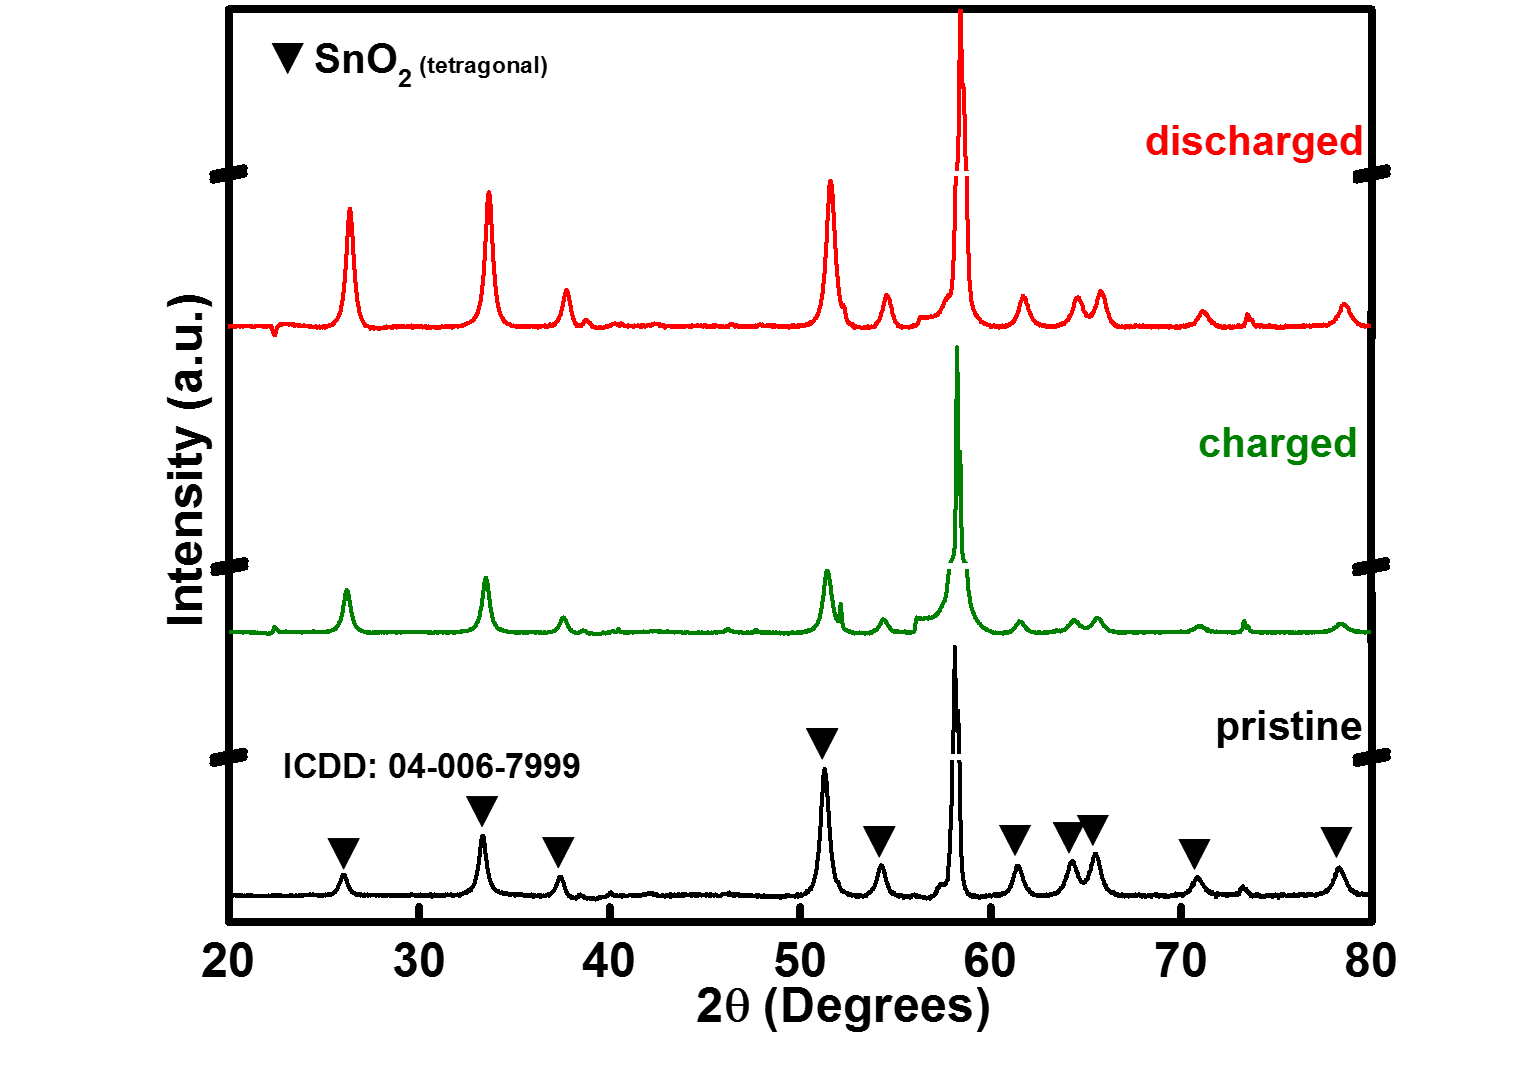
\includegraphics[width=\textwidth]{Figures/chap6fig/SnO2XRD}
    \caption{\textit{Ex-situ} X-ray diffraction patterns of \ce{SnO2} cathode in a pristine (black), charged (green) and discharged (red) state.}
  \label{Figures/chap6fig:SnO2XRD}
\end{figure}

Further analysis such as XPS, is needed to investigate the ongoing mechanism, especially at these voltages. An \textit{ex-situ} XPS analysis of the charged and discharged cathodes would give a lot of information about the changing oxidation states of the active material.


\section{Molybdenum trioxide}

\subsection{Introduction}

 \begin{figure}[th!]
  \centering
  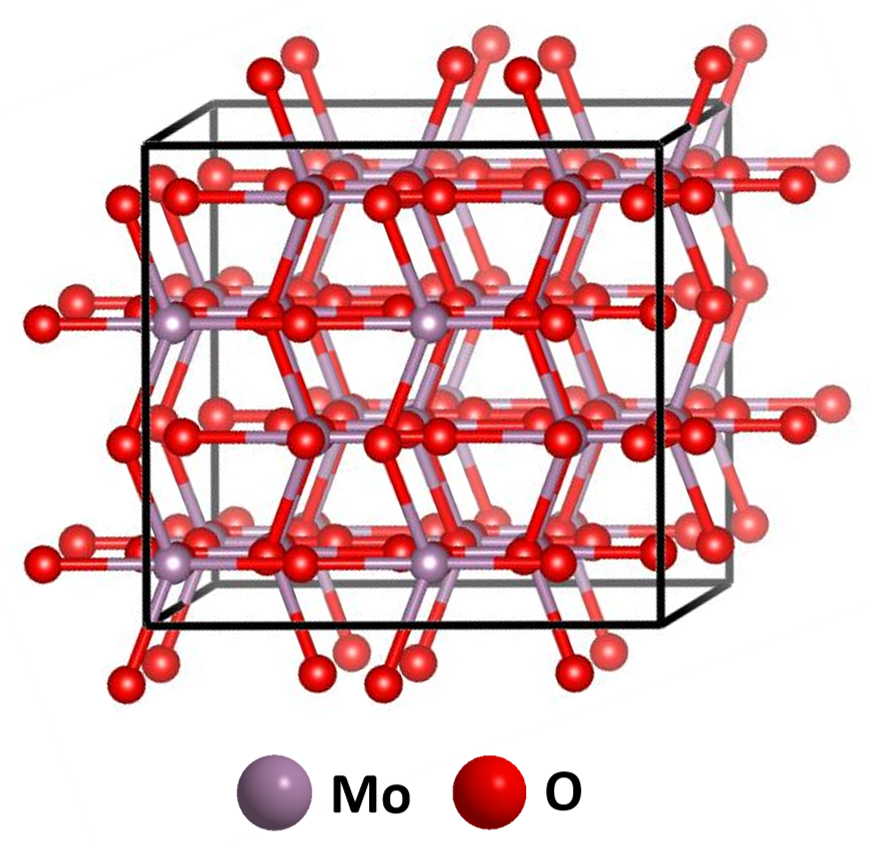
\includegraphics[width=\textwidth]{Figures/chap6fig/MoO3crys}
    \caption{Crystal structure of \ce{MoO3}. a) Tetragonal unit cell with space group P4/nmm and space group number 129. b) Top view of the crystal lattice.}
  \label{Figures/chap6fig:MoO3crys}
\end{figure}

Molybdenum trioxide, \ce{MoO3} is an intermediate formed during production of Mo metal. It consists of layers of \ce{MoO6} octahedra in an orthorhombic crystal held together by covalent forces and Van der Waals forces. Oxygen atoms in back and front of the chain link to other chains to build the layer. When used in lithium-ion, it sometimes undergoes a conversion reaction for lithium storage. High concentrations of unsolvated \ce{Li+} in the oxide host lattice cause significant irreversible morphological changes resulting in poor cell performance \cite{tao,li_theore}. Interestingly, the material has been tested as both cathode and anode. Application of \ce{MoO3} as an anode material is particularly interesting. Since it has a structure with many interstitial sites and layers (Figure \ref{Figures/chap6fig:MoO3crys}, along with a \ce{Mo^{4+}}/\ce{Mo^{5+}} redox couple, it was important that we tested bulk \ce{MoO3} as a cathode material for aluminium-ion batteries.

\begin{center}
 \ce{MoO3} + 6\ce{Li+} + 6\ce{e−} \longrightarrow 3\ce{Li2O} + Mo   
\end{center}

\subsection{Experimental methods}
Molybdenum trioxide (\ce{MoO3} ACS reagent, $\geq$99.5\% was purchased from Sigma-Aldrich and used as received.

\subsection{Results and discussion}
At a high current density of 1500 mA g$^{-1}$ (Figure \ref{Figures/chap6fig:MoO3CDC}a), the \ce{MoO3} cathode afforded a  high specific capacity of $\sim$80 mAh g$^{-1}$ and coulombic efficiency a little above 100\%. After 120 cycles, the cathodic capacity was 75\% retained. Significantly, the charge/discharge curves throughout these cycles overlapped, demonstrating excellent reversibility of the \ce{MoO3} cathode. Constant specific discharge capacities, stable coulombic efficiency, and high average discharge voltage ($\sim$1.45 V) were illustrated within wide range of current densities from 50 mA g$^{-1}$ to 15000 mA g$^{-1}$. 

\begin{figure}[th!]
\centering
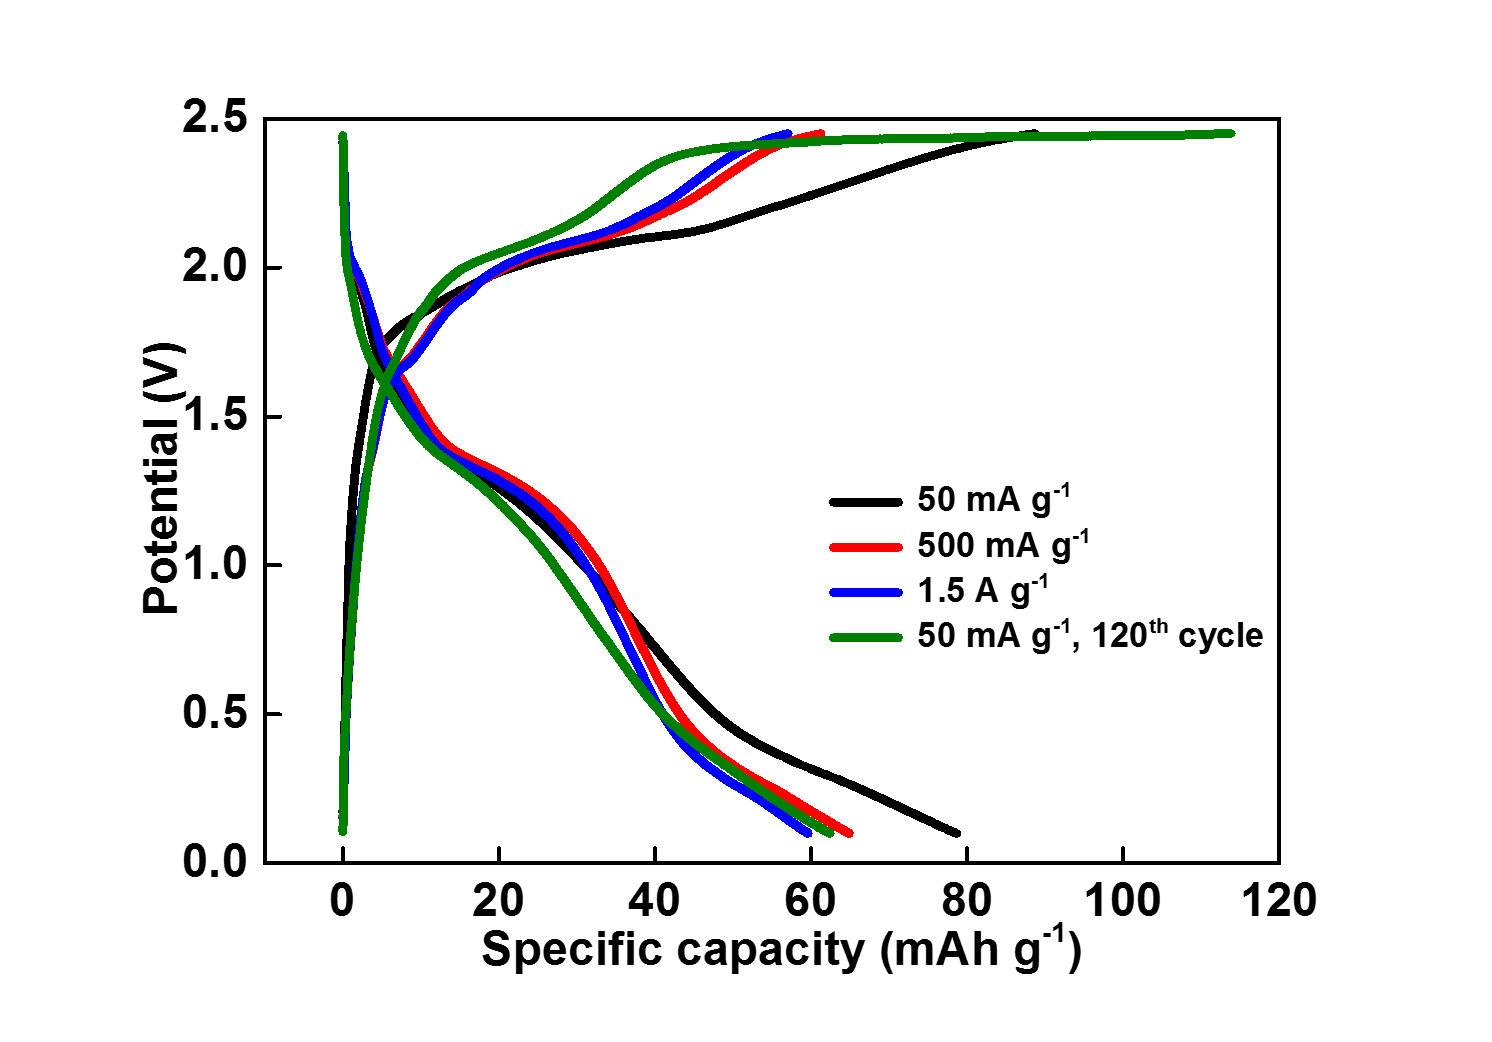
\includegraphics[width=\textwidth]{Figures/chap6fig/MoO3CDCredo}
\caption{Charge/discharge cycles of an Al/\ce{MoO3} cell at various current rates.}
\label{Figures/chap6fig:MoO3CDC}
\end{figure}

Notably, the cathode still retained a reversible high capacity of 60 mAh g$^{-1}$ at an extremely high current density of 1500 mA g$^{-1}$ with clear charging/discharging plateau. This reveals fast intercalation-based chemical redox reaction in the \ce{MoO3} cathode rather than physical adsorption-based electrical double-layer capacitive mechanism. These excellent electrochemical performances, especially high rate capability promise a new generation of energy storage system that can sustainably keep stable energy density of $\sim$85 Wh kg$^{-1}$.


\section{Graphitic Carbon Nitride}

\subsection{Introduction}

\begin{figure}[th!]
\centering
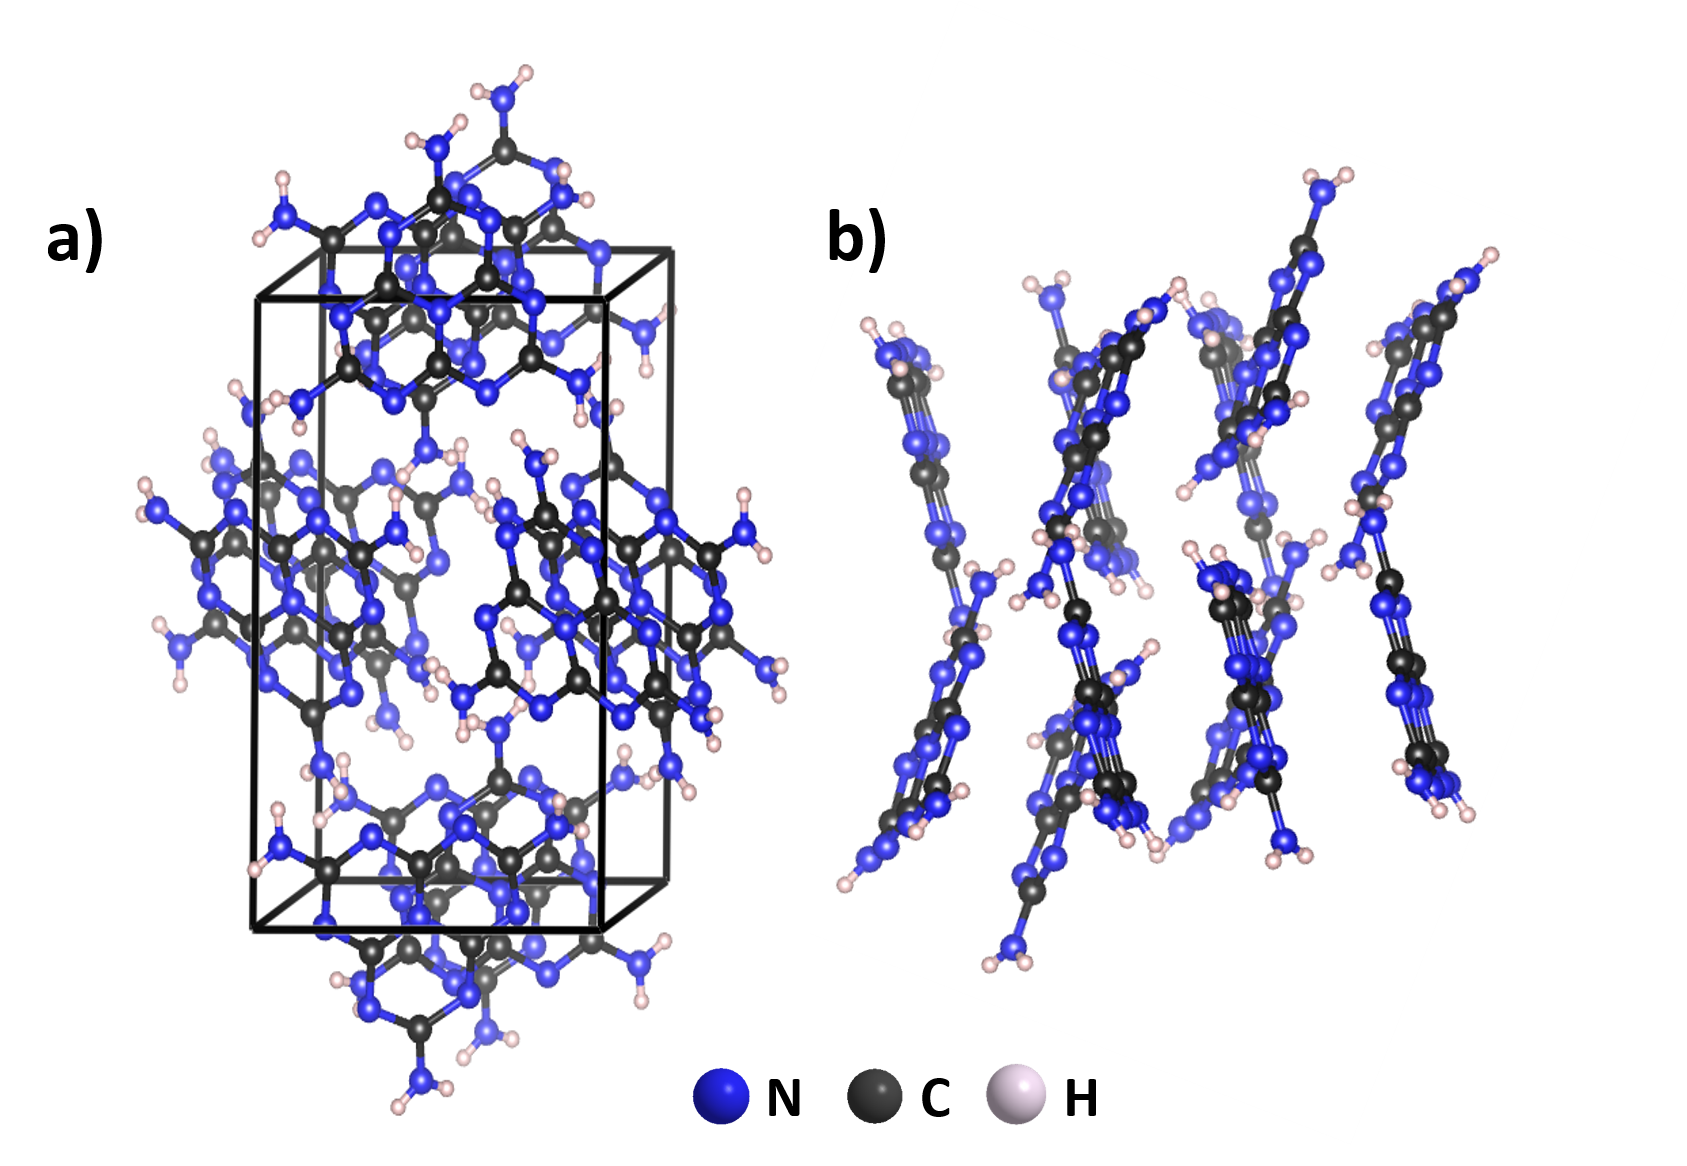
\includegraphics[width=\textwidth]{Figures/chap6fig/C3N4crys}
\caption{.}
\label{Figures/chap6fig:C3N4crys}
\end{figure}
\subsection{Experimental methods}
The material was obtained from the University of Auckland and was used as received. 

\subsection{Results and discussion}
Figure \ref{Figures/chap6fig:C3N4cdc} shows charge/discharge curves and charge/discharge capacities of the rechargeable Al cell with the \ce{C3N4} positive electrode at $\sim$80 mAh g$^{-1}$. The discharge capacity at the first cycle was 100 mAh g$^{-1}$, whereas that at the 120$^{th}$ cycle was below $\sim$80 mAh g$^{-1}$. Charge and discharge capacities were almost the same, suggesting that the rechargeable Al cell showed high coulombic efficiency. Figure \ref{Figures/chap6fig:C3N4cdc}a shows discharge capacities with different current densities. When discharge current was decreased to 50, capacity increased to 100 mAh g$^{-1}$, whereas at 1500 mA g$^{-1}$, capacity was below 20 mAh g$^{-1}$. In conclusion, \ce{C3N4} showed decent electrochemical activity for reversible ion intercalation and extraction with good cycle stability. 

\begin{figure}[th!]
\centering
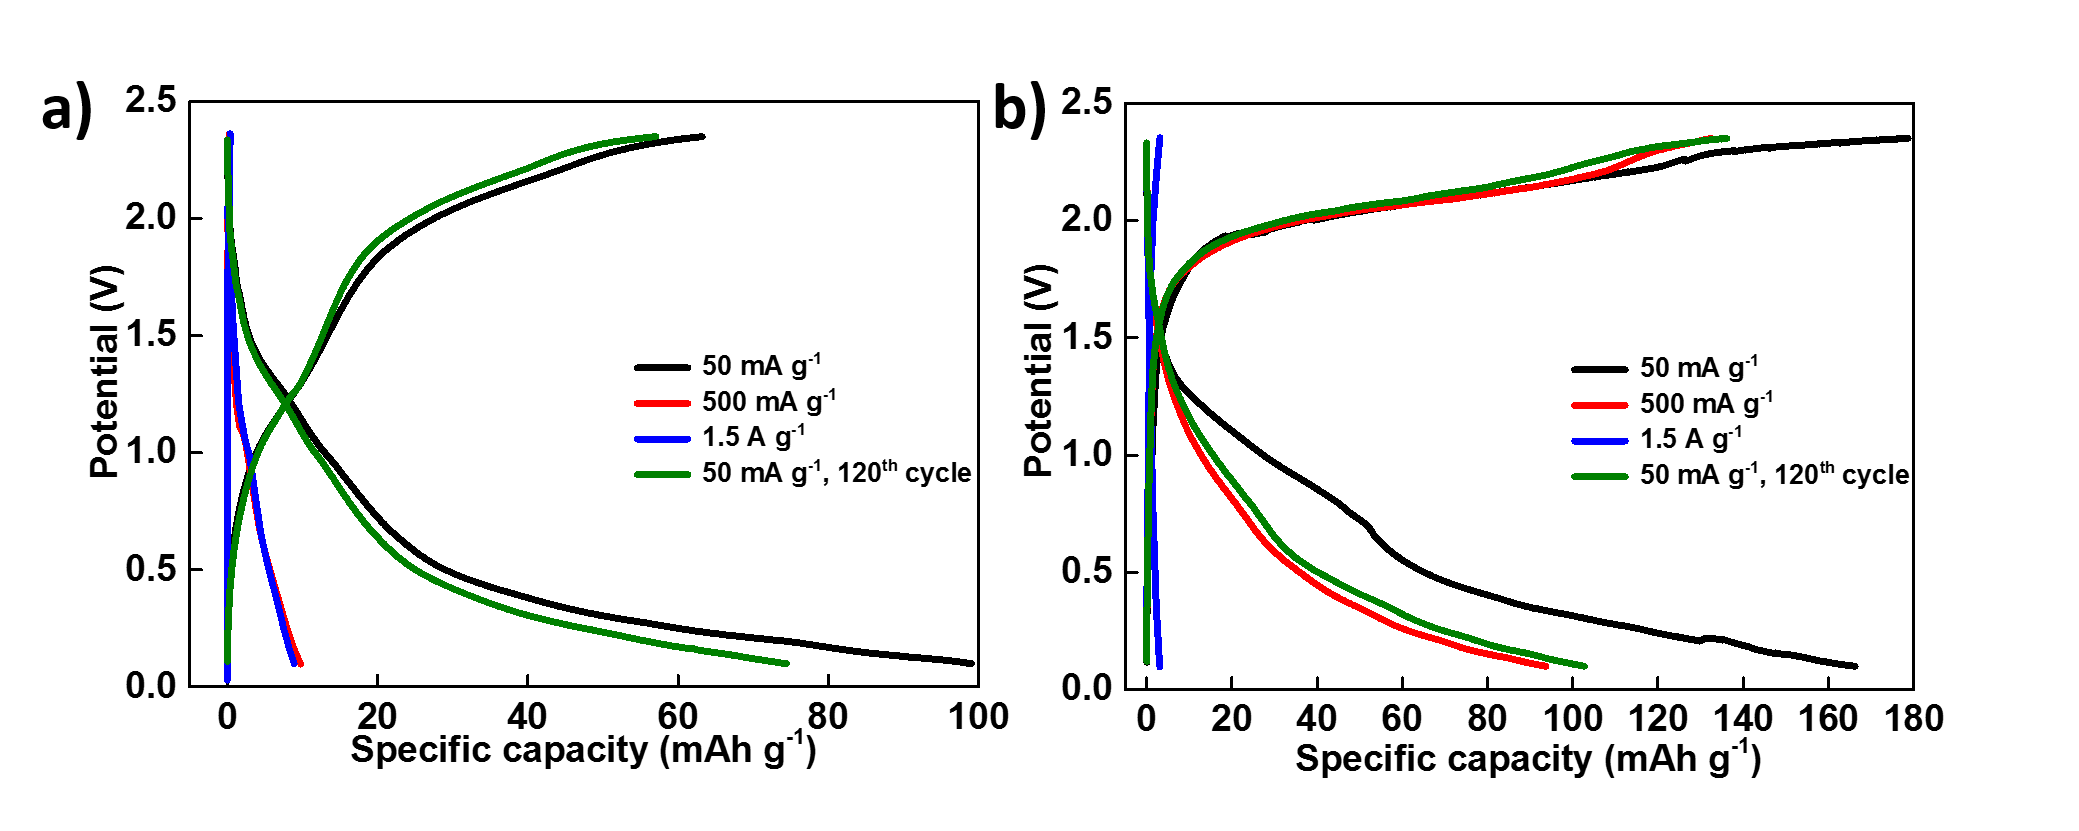
\includegraphics[width=\textwidth]{Figures/chap6fig/C3N4cdc}
\caption{Charge/discharge cycles of an Al/\ce{MoO3} cell at various current rates.}
\label{Figures/chap6fig:C3N4cdc}
\end{figure}

\section{Prussian blue}

\subsection{Introduction}

 \begin{figure}[tbh!]
  \centering
  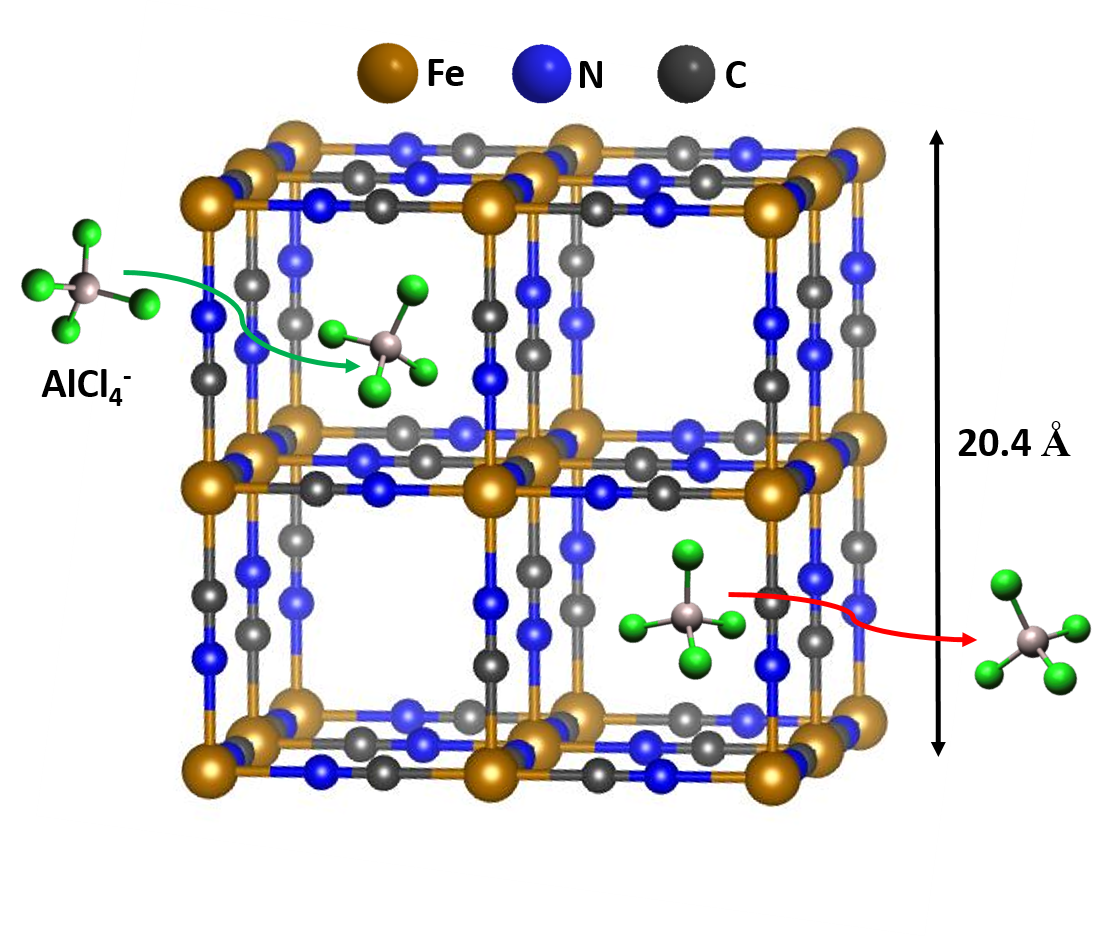
\includegraphics[width=\textwidth]{Figures/chap6fig/pbcrys}
    \caption{Crystal structure of prussian blue a) Tetragonal unit cell with space group P4/nmm and space group number 129. b) Top view of the crystal lattice.}
  \label{Figures/chap6fig:pbcrys}
\end{figure}

Prussian blue was originally commercialised in the dye industry. Since, it has been used for electrolysis, thermal power generation and energy storage. It has a face-centred cubic lattice with an open framework as shown in Figure \ref{Figures/chap6fig:pbcrys}, which helps in insertion of ions in the sub-cages. Its structure is very stable and has a number of redox sites present. Each molecular formula contains two redox centres \ce{M+2}/\ce{M3+}, where M is any transition metal (Fe, Co, Ni, Mn, Cu, Zn). It reaches 2\ce{e-} redox capacity after reversibly intercalating 2 monovalent alkali ions per molecular unit. Presence of large lattice interstices and ionic channels renders a high specific capacity. 

\subsection{Experimental methods}
\subsection{Results and discussion}
The first cycle galvanostatic charge–discharge curve of Al–prussian blue cells exhibited voltage plateaus at 1.8, 1.2 V and 0.6 V with a capacity of $\sim$140 mAh g. To investigate the rate capabilities of the battery, the cell was charged and discharged at various current densities (Figure \ref{Figures/chap6fig:pbCDC2}a) ranging from 50-1500 mA g$^{-1}$. the cycle performances and coulombic efficiency were investigated with a cut-off voltage between 2.35 V and 0.1 V at a current density of 50 mA g$^{-1}$ over 180 cycles, as shown in Figure \ref{Figures/chap6fig:pbCDC2}b. It can be seen that the capacity decreases significantly (45\%) over the first 20 cycles, Figure \ref{Figures/chap6fig:pbCDC2}b. The discharge capacity for the first cycle is 140 mAh g$^{-1}$, exhibiting multiple discharge voltage plateaus ranging from 1.9 V to 0.5 V. With the increase in current density, the capacity of the Al-ion battery gradually decreased to 5 mAh g$^{-1}$. It can be found that although capacities remained quite stable after initial cycling, coulombic efficiency showed a slightly decreasing trend, and decreased from 150 to $\sim$80\% after 180 cycles. 

 \begin{figure}[tbh!]
  \centering
  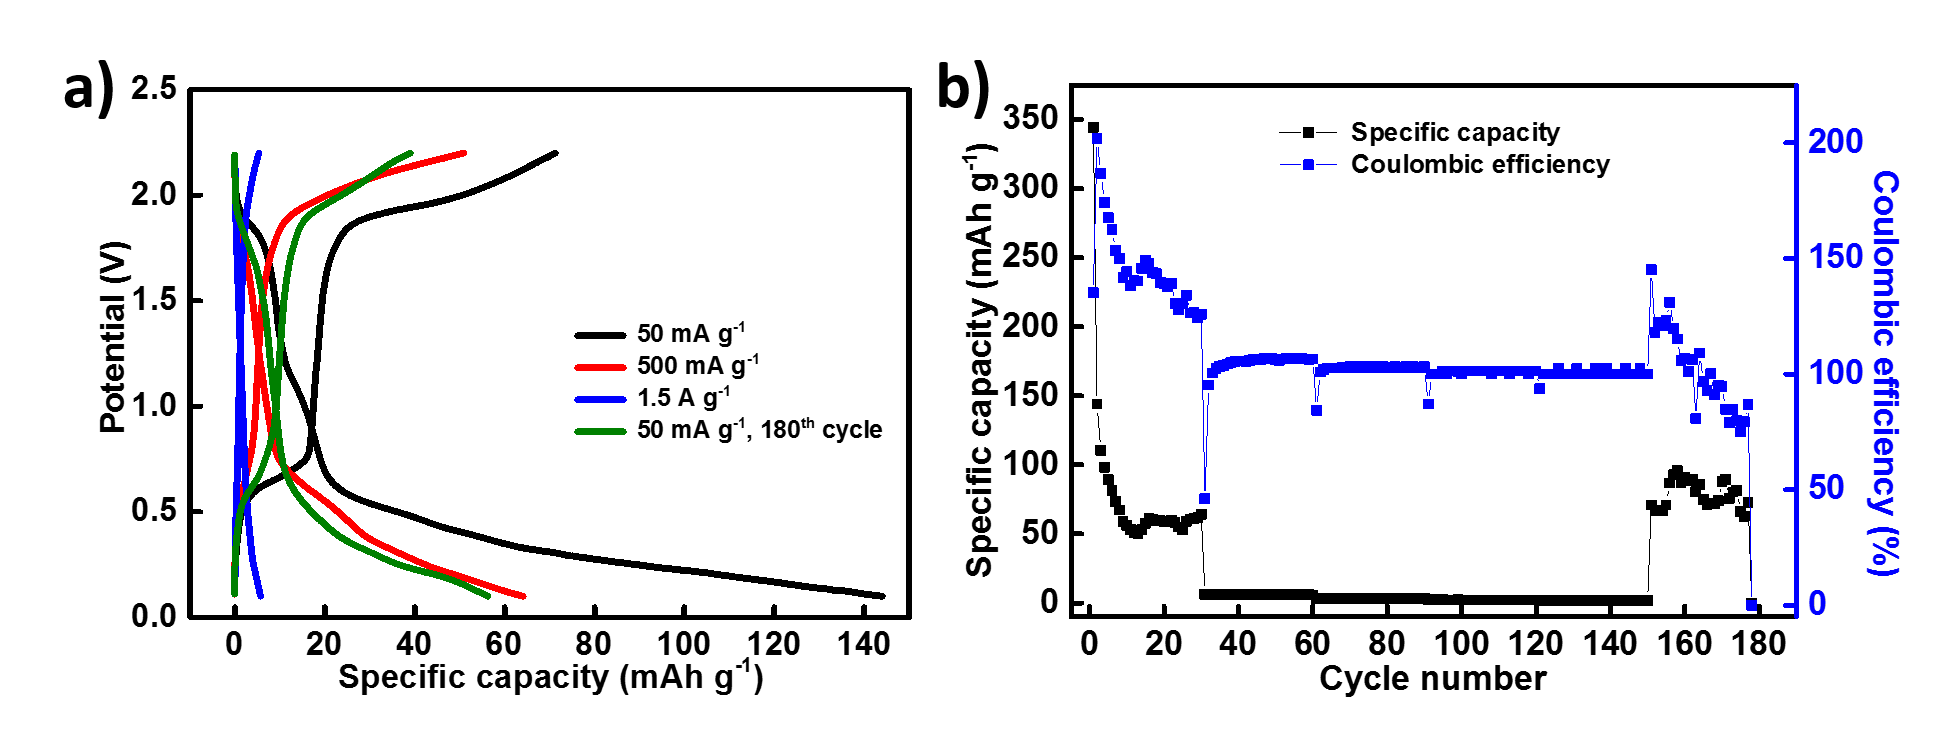
\includegraphics[width=\textwidth]{Figures/chap6fig/pbCDC2}
    \caption{Galvanostatic cycle test of an Al/\ce{C19Fe7N18} cell in a two-electrode setup at various current rates.}
  \label{Figures/chap6fig:pbCDC2}
\end{figure}

\subsection{Conclusion and future outlook}
Significant crystallography and voltammetry studies are underway to understand intercalation of aluminium into V2O5 and other layered oxides. These studies will help
shed light on the effect of variables such as the cell current
density and electrolyte formulation on the coulombic efficiency
and practical specific energy achievable in the Al-ion battery. As in the case of Li-ion secondary batteries, we anticipate significant opportunities for nanoscale engineering and chemical design of the Al-ion battery cathode to increase the overall cell potential. Additionally, we anticipate as significant efforts to pioneer ionic liquid and
